%!TEX root=masterproef.tex

\chapter{Software-attestatie}
\label{appendix:attestation}

In deze bijlage bekijken we een voorbeeld van software-attestatie, meer
specifiek het ICE-algoritme \citep{seshadri2006scuba, seshadri2008sake} en
evalueren de mogelijkheden en beperkingen.

Figuur \ref{fig:attestation-process} illustreert de werking van
software-attestatie en toont hoe een wijziging door een aanvaller zich
propageert van het geheugen naar de checksum.

\begin{figure}[ht] \centering
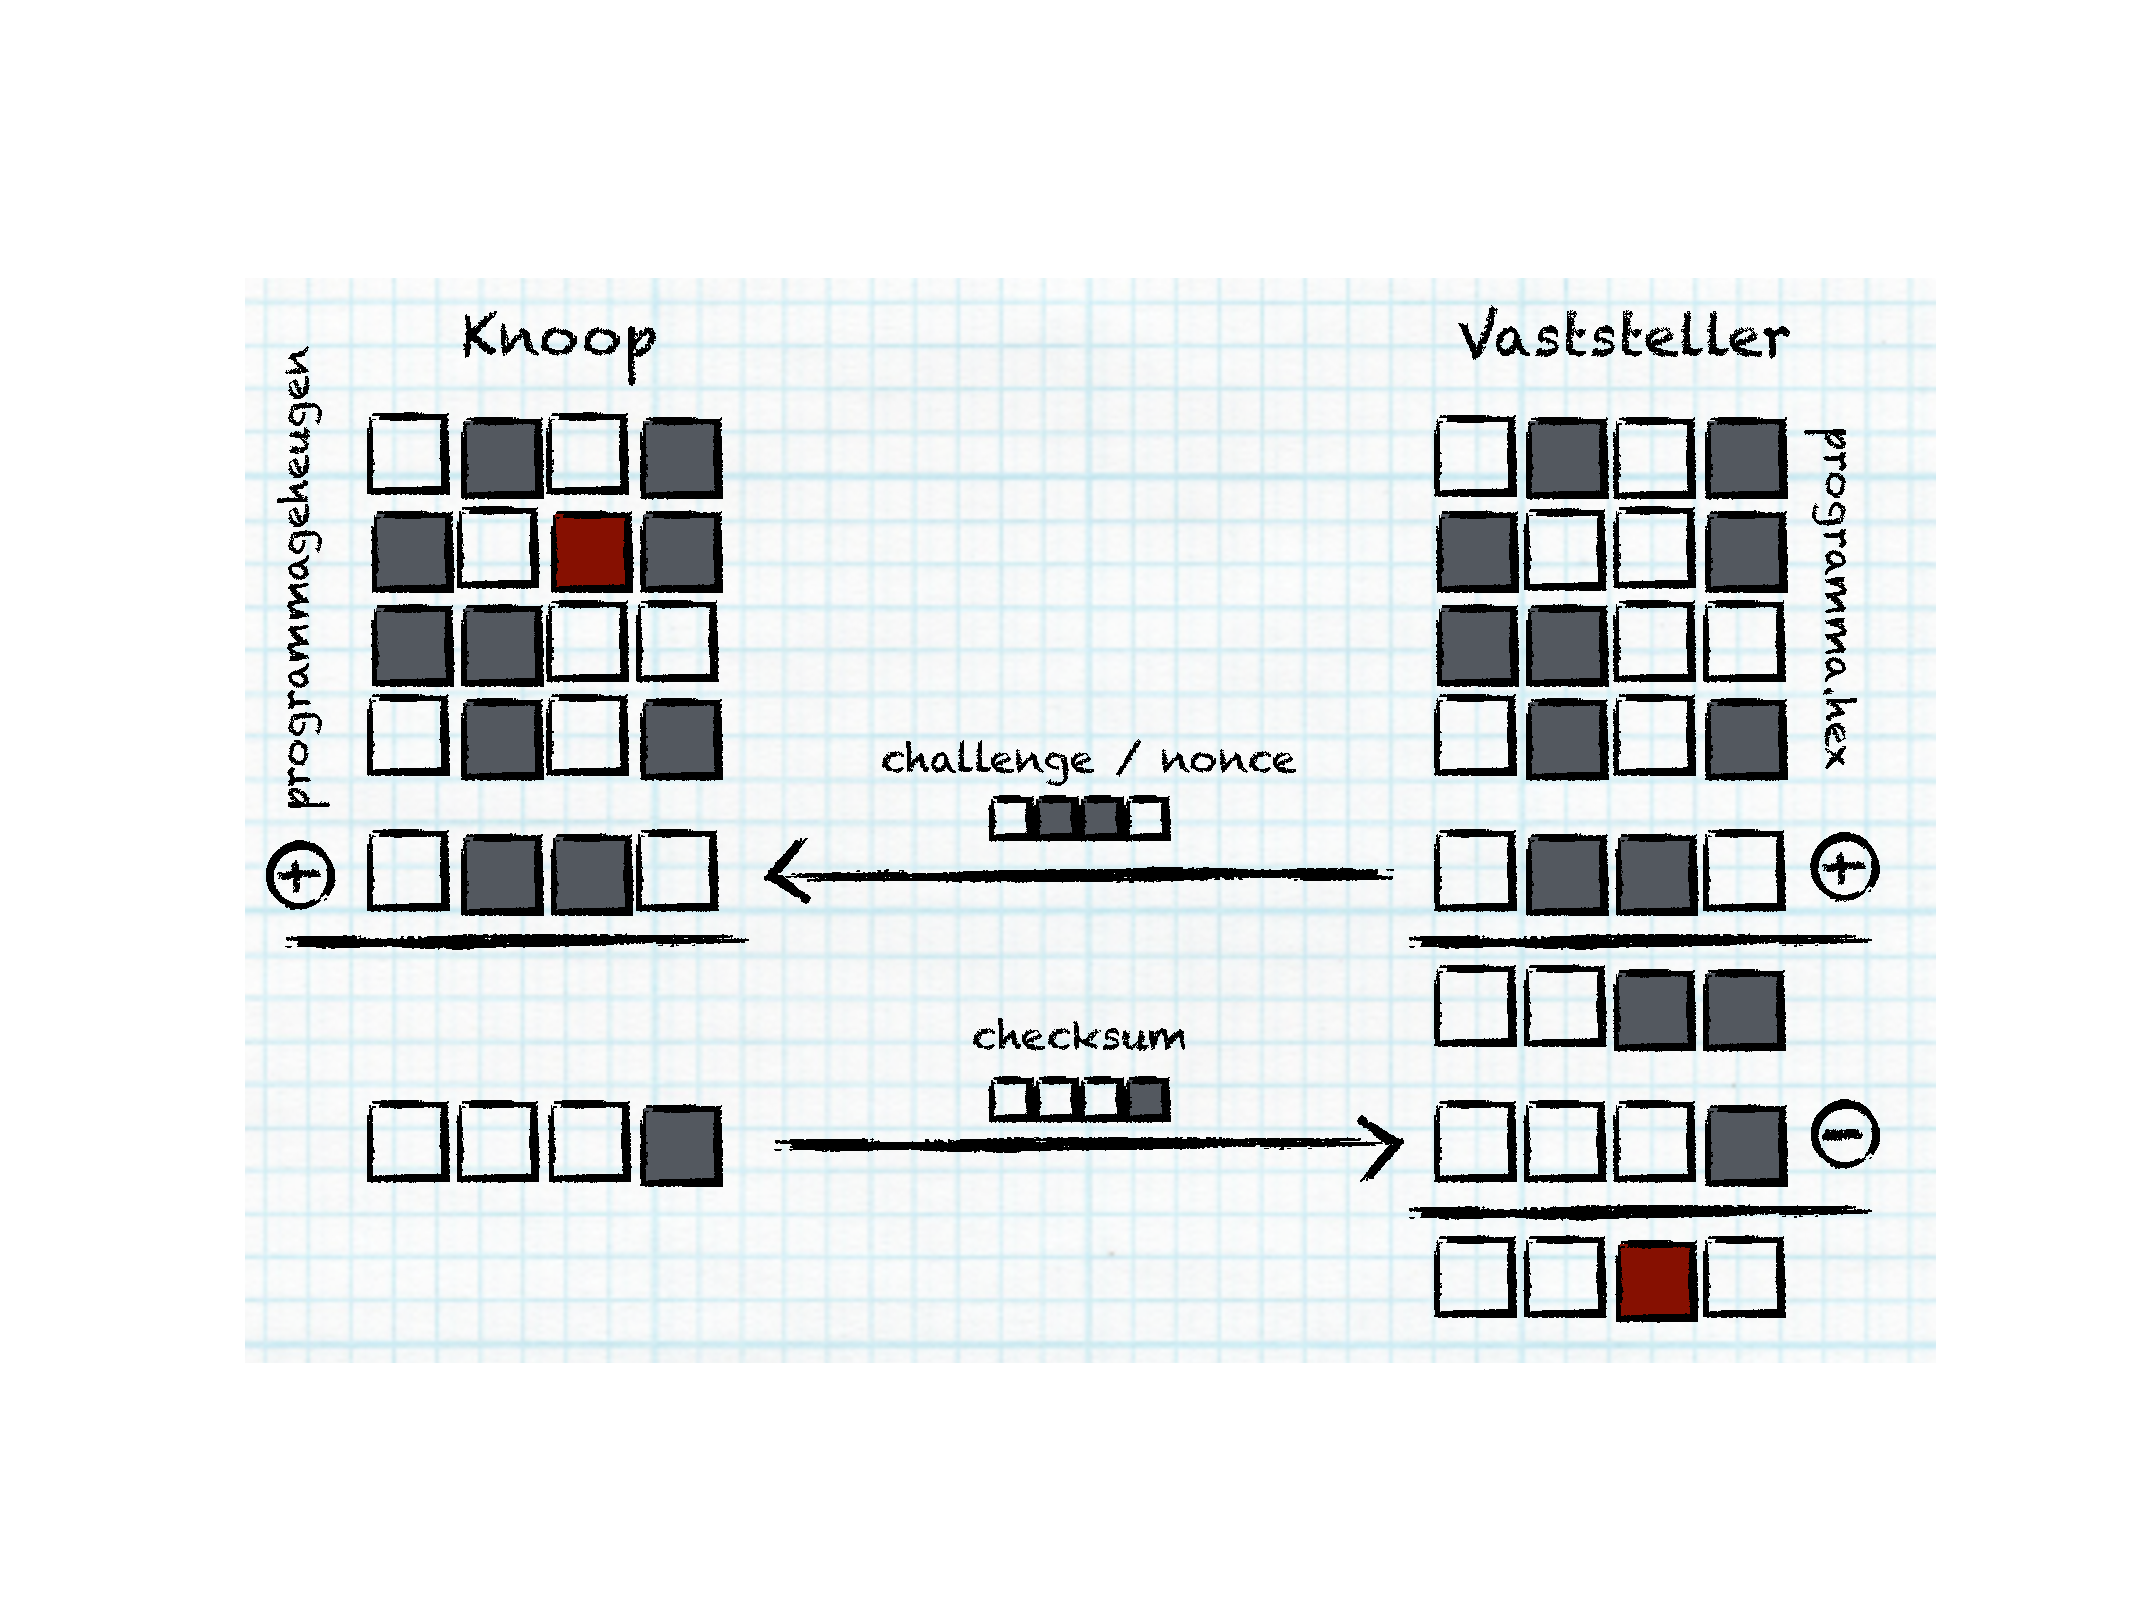
\includegraphics[width=0.9\linewidth]{resources/attestation-process.pdf}
\caption[De werking van software-attestatie]{De werking van
software-attestatie: een aanvaller heeft een wijziging (rood gekleurd vlak in
de voorstelling van het geheugen van de knoop) kunnen aanbrengen in de
programmacode op een knoop. Deze wijziging propageert zich in de
\emph{checksum} en wordt door de vaststeller opgemerkt.}
\label{fig:attestation-process} \end{figure}

\section{Implementaties}

SWATT werd voorgesteld in \citep{seshadri2004swatt} en is een
attestatieprocedure die een \emph{checksum} berekent over nagenoeg alle
geheugenlocaties, echter wel in willekeurige volgorde. Anderzijds houdt SWATT
ook rekening met de tijd die de attestatie routine op de knoop nodig heeft om
de \emph{checksum} te berekenen. Indien een aanvaller code zou toevoegen om de
werking van de attestatie routine te verstoren, zou dit op te merken zijn in de
vorm van een vertraging van het antwoord aan de vaststeller.

Met SCUBA in \citep{seshadri2006scuba} en SAKE in \citep{seshadri2008sake} werd
verder gebouwd op SWATT met het oog op een beveiligde distributie van
programmacode en het veilig uitwisselen van sleutels. Samen met SCUBA en SAKE
werd ook \emph{Indisputable Code Execution} (ICE) ge\"introduceerd. Daar waar
SWATT gericht is op inhoudelijke integriteit, voegt ICE hieraan ook de garantie
van een niet-aangetaste uitvoering van programma's toe en laat toe om beperkte
regio's van het geheugen te benaderen.

Op deze manier kan nu bovenop de attestatie van het geheugen van een knoop ook
functionaliteit aangeroepen worden, waarvan de werking gegarandeerd veilig is.
Zo wordt het mogelijk om nieuwe code te installeren of gedeelde geheimen uit te
wisselen.

ICE realiseert dit door een \emph{checksum} te berekenen over de geheugenregio
waar de attestatieroutine zich bevindt, over de regio waar het uit te voeren
programma zich bevindt en van de staat van de processor. Hierdoor ontstaat er
een garantie dat de attestatie correct verloopt, dat het uit te voeren
programma geen onbekende code bevat en dat de omgeving waarin de attestatie en
het programma uitgevoerd worden gegarandeerd niet aangetast wordt.

Een belangrijke eigenschap van ICE is dat de attestatieroutine de processor in
een \emph{veilige} staat brengt door geen \emph{interrupts} toe te laten.
Hierdoor kan de werking van de attestatieroutine niet onderbroken of gewijzigd
worden. Na succesvolle attestatie zal het geattesteerde programma in dezelfde
veilige omstandigheden als de ICE routine uitgevoerd worden.

\section{Evaluatie}

SWATT en ICE werden in \citep{castelluccia2009difficulty} onder de loep genomen
en verschillende manieren om deze vormen van integriteitscontrole te omzeilen
werden voorgesteld. Ondanks het feit dat verschillende interessante aspecten
van de attestatietechnieken werden belicht, werden te snel veronderstellingen
rond beide implementaties gemaakt en werd in \citep{perrig2010refutation} een
weerwoord gegeven.

Desalniettemin zijn de voorgestelde ontwijkingstechnieken zeer interessante
voorbeelden van de mogelijkheden die een aanvaller heeft tegen
software-attestatie.

\subsection{Vrij geheugen}

De fundamentele manier om de attestatiecode te omzeilen bestaat er in om de
opgevraagde geheugenadressen te controleren en indien ze verwijzen naar
plaatsen waar zich niet-originele code bevindt, deze te herschrijven naar
adressen waar de originele code zich bevindt.

Aangezien het merendeel van het programmageheugen op een knoop typisch leeg is,
kan de aanvaller zijn benodigde code verbergen in zo'n stuk leeg geheugen. Mits
zorgvuldige keuze van deze locatie, kan het controleren van en verwijzen naar
een andere locatie zich beperken tot de manipulatie van \'e\'en enkele bit in
het adres. Deze techniek wordt ook wel een geheugenschaduwende aanval genoemd.

Om het probleem van een leeg programmageheugen en de bijhorende uitnodiging aan
het adres van de aanvaller om zich hier eenvoudig te kunnen verschuilen, aan te
pakken, stellen o.a. \citep{yang2007distributed,seshadri2008sake} voor dat dit
geheugen opgevuld wordt met willekeurige waarden. Op deze manier heeft de
aanvaller geen vrije ruimte om zijn code in te plaatsen.

Deze willekeurige waarden kunnen zo opgesteld worden dat ze niet verkleind
kunnen worden. Dit kan echter niet gegarandeerd worden van de eigenlijke
programmacode. Deze kan typisch wel nog verkleind en in die vorm opgeslagen
worden, waardoor er mogelijk voldoende ruimte vrijkomt voor de code van de
aanvaller. Op het ogenblik van attestatie kan deze oorspronkelijke code dan,
indien nodig, terug hersteld worden.

Indien deze eenvoudige technieken toch niet voldoende ruimte zouden bieden, kan
er nog altijd gekeken worden naar het datageheugen. We merken immers op dat
nagenoeg alle vormen van attestatie alleen toegepast worden op het
programmageheugen. Het datageheugen is te veranderlijk en kan niet volledig
gekend zijn door de vaststeller. Hierdoor wordt dit datageheugen natuurlijk het
volgende mogelijke aandachtspunt voor de aanvaller. Ondanks het feit dat op een
\mcu het datageheugen veelal niet kan uitgevoerd worden, blijft het mogelijk om
programmacode in het datageheugen op te slagen en te kopi\"eren naar het
programmageheugen.

\subsection{Een rootkit}

De \emph{rootkit} voorgesteld in \citep{castelluccia2009difficulty} misbruikt
dit vrije geheugen. Door middel van \emph{Return Operation Programming} (ROP),
o.a. beschreven in \citep{prandini2012return}, kan een aanvaller met eerste
aanknopingspunt of \emph{haak} bij aanvang van de attestatiecode in het
programmageheugen, zijn eigen rootkit uit het programmageheugen laten
verwijderen. Na deze operatie is het programmageheugen opnieuw intact en zal de
originele attestatieroutine een positief resultaat opleveren. Maar de eerste
haak heeft er ook voor gezorgd dat bij terugkeer uit de attestatieroutine een
tweede haak geplaatst is die op zijn beurt de rootkit en de initi\"ele haak
opnieuw door middel van ROP-instructies installeert. Figuur
\ref{fig:attestation-rootkit} toont deze werking.

\begin{figure}[ht]
  \centering
  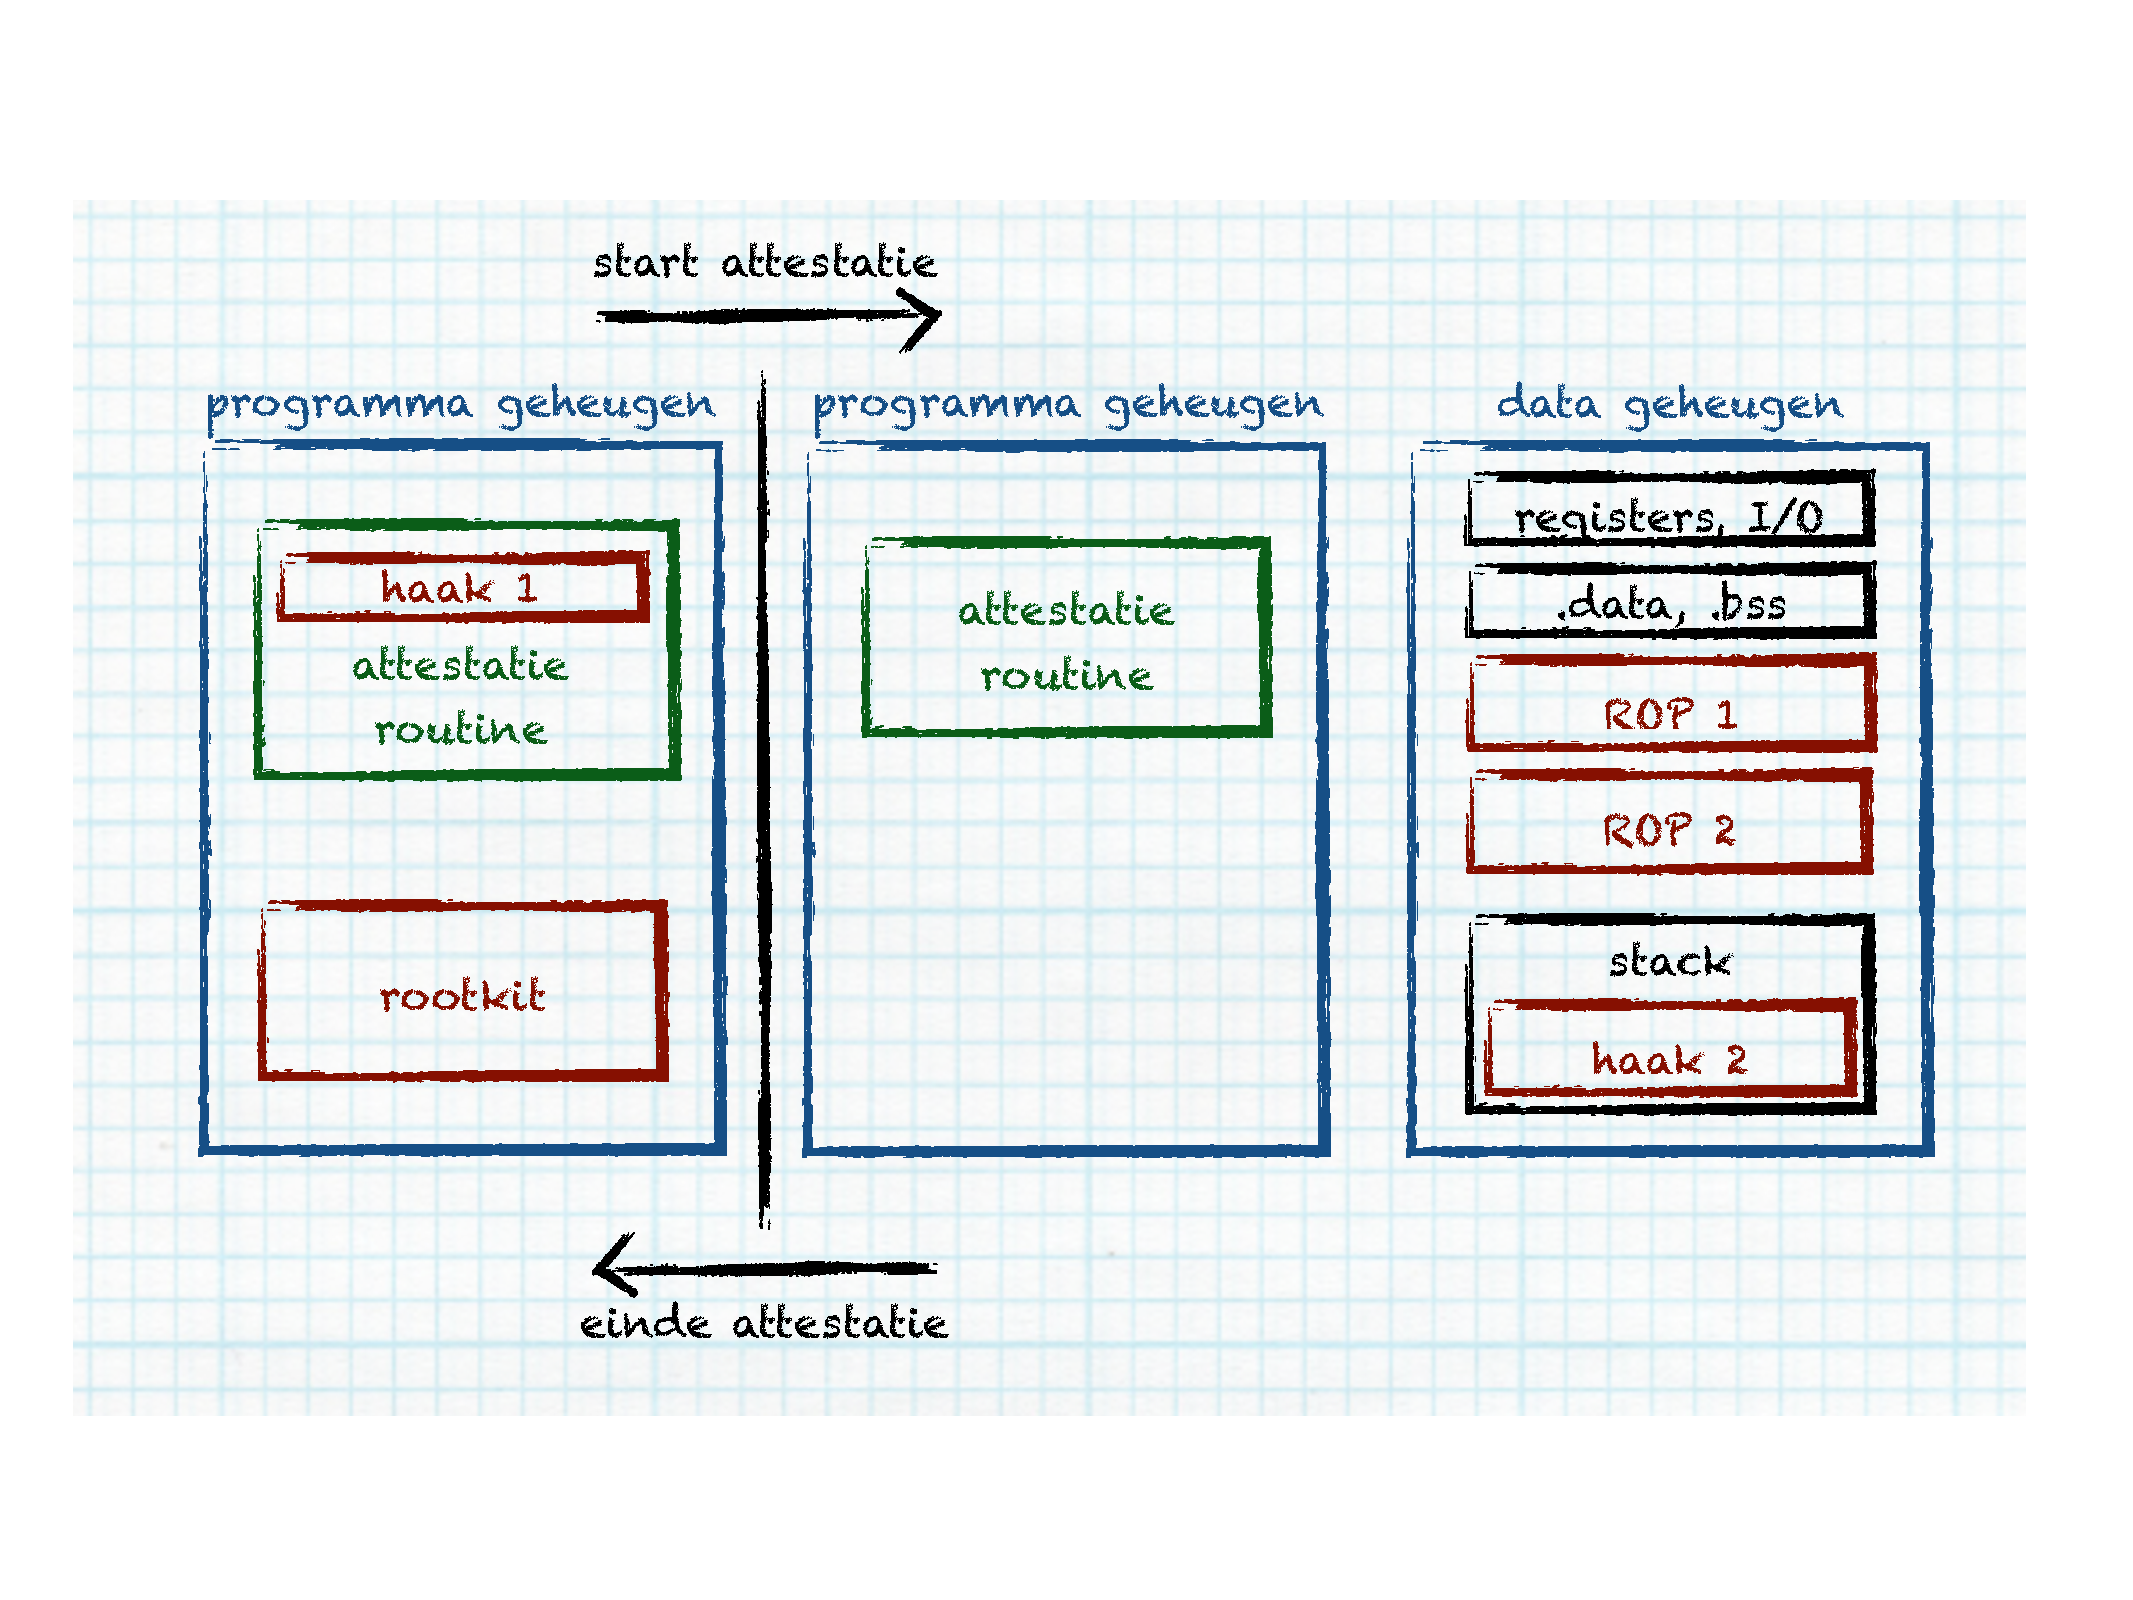
\includegraphics[width=0.9\linewidth]{resources/attestation-rootkit.pdf}
  \caption{De werking van een attestatie-ontwijkende rootkit}
  \label{fig:attestation-rootkit}
\end{figure}

Het verbergen van de rootkit en het herstellen van het programmageheugen in
zijn oorspronkelijke staat blijkt slechts een overhead van ongeveer 0.3\% op te
leveren t.o.v. bv. de attestatietechniek voorgesteld in
\citep{seshadri2004swatt}. Deze techniek controleert tevens de tijd dat de
attestatieroutine nodig had om de checksum te berekenen. Indien deze te lang
duurt dan schrijft SWATT dit toe aan de overhead ge\"introduceerd door
mogelijke kwaadaardige code. Een verhoging met 0.3\% is mogelijk te weinig om
tot deze conclusie te komen.

Deze aanval richt zich nu louter op de attestatieroutine, maar zoals in
\citep{perrig2010refutation} aangegeven wordt, is SWATT slechts een deel van
een volledige software-attestatie en focust zich op het effectief attesteren
van code in het geheugen, niet op de omringende context. In een volledige
opstelling zou een attestatieprocedure het terugkeeradres op de stack mee
kunnen nemen in de attestatie.

\subsection{Maatregelen}

\citep{castelluccia2009difficulty} beschrijven zelf enkele mogelijke pistes
waarmee een attestatieroutine zichzelf zou kunnen beschermen tegen een
dergelijke rootkit. Een voorbeeld is het leegmaken van het datageheugen en
vervolgens, zonder een terugkeeroperatie uit te voeren - waardoor de tweede
haak vermeden wordt - de knoop te herstarten. Het verwijderen van alle gegevens
en het herstarten van een knoop bij elk attestatieverzoek kan, afhankelijk van
de functionaliteit die de knoop aanbiedt, in de meeste gevallen niet wenselijk
zijn. Dit euvel kan eventueel wel ondervangen worden door het wegschrijven van
deze gegevens naar een EEPROM, een geheugen dat de opgeslagen gegevens bewaart
bij herstarten.

\subsection{Het algoritme}

Naast SWATT werd in \citep{castelluccia2009difficulty} ook een
aanvalsmogelijkheid tegen ICE voorgesteld. Het \emph{checksum}-algoritme van
ICE is zo geconstrueerd dat het niet mogelijk is om bij elke geheugentoegang na
te gaan of er een doorverwijzing moet gebeuren of niet. Het is echter wel
mogelijk om een consequente bit-wijziging te doen, zonder voorafgaande test.

Algoritme \ref{alg:attestation-ice} toont het \emph{checksum}-algoritme. De
eigenlijke berekening vanaf regel 4 bestaat uit een strikte afwisseling van
16-bit-optellingen zonder overdracht en XOR-operaties ($\oplus$).

\begin{algorithm}
\begin{algorithmic}[1]
  \Require{y, het aantal iteraties dat de verificatie routine uitvoert}
  \For{$l = y \: to \: 0$}
    \Let{$x$}{$x + (x^2 \vee 5) mod 2^{16}$} \Comment{T functie voor $0 < x < 2^{16}$}
    \Let{$daddr$}{$(daddr \: \oplus \: x ) \wedge MASK) + code\_start$} \Comment{adres gebaseerd op $x$.}
    \Let{$C_j$}{$C_j + PC$}   \Comment{Program Counter}
    \Let{$C_j$}{$C_j \oplus mem[daddr]$}  \Comment{het willekeurige geheugenadres}
    \Let{$C_j$}{$C_j + l$}
    \Let{$C_j$}{$C_j \oplus C_{j-1}$}
    \Let{$C_j$}{$C_j + x$}
    \Let{$C_j$}{$C_j \oplus daddr$}
    \Let{$C_j$}{$C_j + C_{j-2}$}
    \Let{$C_j$}{$C_j \oplus SR$}    \Comment{Status register}
    \Let{$C_j$}{\Call{rotate\_left}{$C_j$}}
    \Let{j}{$(j+1)\: mod \: 10$}
  \EndFor
\end{algorithmic}
\caption{ICE pseudo-code\label{alg:attestation-ice}}
\end{algorithm}

Een mogelijke aanval op ICE bestaat er in om twee wijzigingen aan te brengen
die elkaar opheffen, waardoor eenzelfde checksum berekend wordt. Praktisch is
het mogelijk om de meest betekenisvolle bit van de programmateller
(\emph{program counter}) (PC) en van de waarde van de opgehaalde
geheugenlocatie te wisselen. Door de opeenvolging van de optelling en de
XOR-operatie zullen deze elkaar opheffen, zoals getoond wordt in
\ref{eq:attestation-ice} en \ref{eq:attestation-ice-bitflip}, waarin een
voorbeeld wordt gegeven met 8-bit argumenten.

\begin{equation} \label{eq:attestation-ice}
\begin{array}{cccccccccc}
       & c_{j-1}    & 1 &	0 &	1 &	0 &	1 &	1 &	1 &	0 \\
+	     & PC	        & 0	& 1	& 1	& 0	& 1	& 0	& 1	& 1 \\
\cline{1-10}
       &            &	0	& 0	& 0	& 1	& 1	& 0	& 0	& 1 \\
\oplus &	mem[addr]	& 0	& 1	& 1 &	0	& 1	& 1	& 0	& 1 \\
\cline{1-10}
       &            &	0	& 1	& 1	& 1	& 0	& 1	& 0	& 0 \\
\end{array}
\end{equation}

\begin{equation} \label{eq:attestation-ice-bitflip}
\begin{array}{cccccccccc}
       & c_{j-1}    & 1 &	0 &	1 &	0 &	1 &	1 &	1 &	0 \\
+	     & PC	        & \bm{1}	& 1	& 1	& 0	& 1	& 0	& 1	& 1 \\
\cline{1-10}
       &            &	\bm{1}	& 0	& 0	& 1	& 1	& 0	& 0	& 1 \\
\oplus &	mem[addr]	& \bm{1}	& 1	& 1 &	0	& 1	& 1	& 0	& 1 \\
\cline{1-10}
       &            &	0	& 1	& 1	& 1	& 0	& 1	& 0	& 0 \\
\end{array}
\end{equation}

Het resultaat van deze minimale aanpassingen is dat er zich een situatie
voordoet zoals weergegeven in figuur \ref{fig:attestation-ice-copy}. De
aanvaller kan zijn eigen aangepaste kopie van de ICE-routine laten uitvoeren.
De geattesteerde regio bevindt zich echter elders, waardoor de routine niet
meer zelfattesterend is en zijn beginsel verliest.

\begin{figure}[ht]
  \centering
  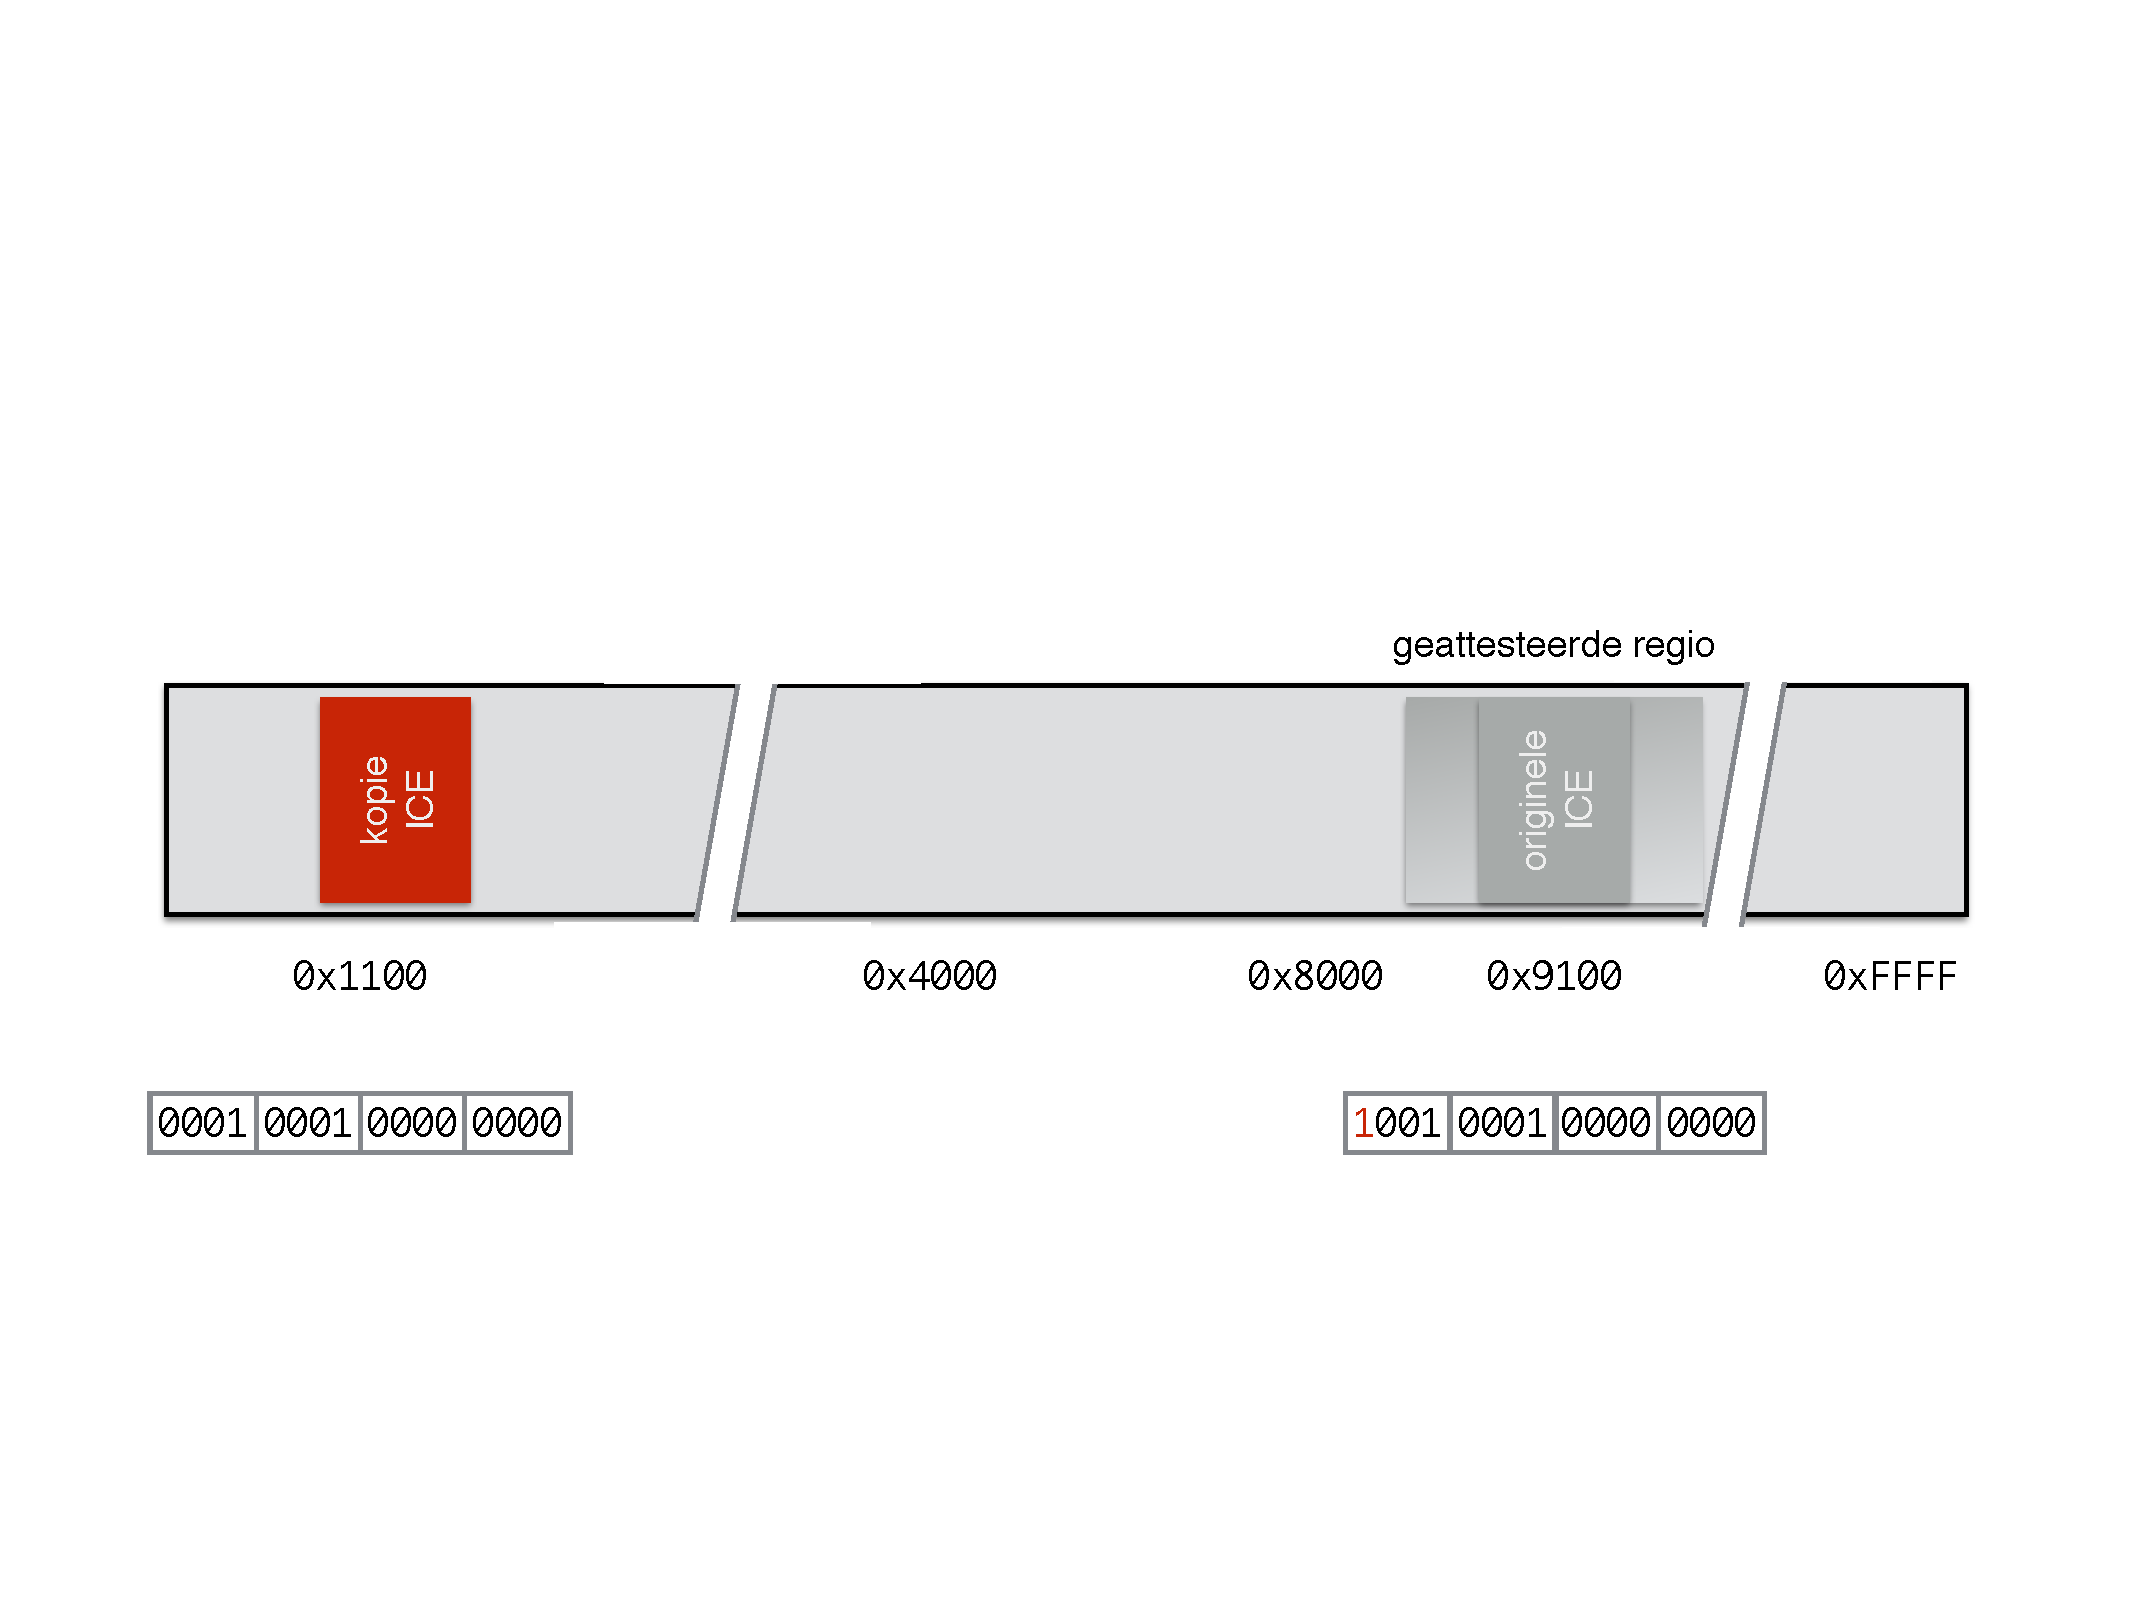
\includegraphics[width=0.9\linewidth]{resources/attestation-ice-copy.pdf}
  \caption[Omzeilen van ICE-gebaseerde software-attestatie]{De legitieme
  ICE-routine is opgeslagen op adres 0x9100 en een aangepaste kopie op adres
  0x1100. Deze twee adressen verschillen slechts in hun meest betekenisvolle
  bit. De aanvaller kan zijn code gebruiken \'en slagen voor de attestatie.}
  \label{fig:attestation-ice-copy}
\end{figure}

In \citep{perrig2010refutation} bevestigen de auteurs van ICE dat er fouten
zijn geslopen in de definitie van ICE en dat ze opportuniteiten hebben laten
liggen om deze aanval tegen te gaan.

\subsubsection*{Trusted Platform Module - TPM}

In voorgaande paragrafen, lag de nadruk op het software-aspect van attestatie.
Voor \mcu's met beperkte mogelijkheden, is het belangrijk om zo effici\"ent
mogelijk om te springen met energie. Ook de kostprijs is een belangrijke
factor, aangezien bijkomende kosten per knoop snel kunnen oplopen in het kader
van een volledig netwerk.

Software biedt in dit laatste geval dan logischerwijs een positief economisch
antwoord. Het is echter ook mogelijk om voor attestatie beroep te doen op
hardware. Daar waar een eenvoudige \mcu zich niet kan beschermen tegen fysieke
aanvallen, is het wel mogelijk om specifieke hardware te cre\"eren die
hermetisch afgesloten is.

Een voorbeeld hiervan is de \emph{Trusted Platform Module} (TPM), van de
\emph{Trusted Platform Group}. Dit is een specificatie die toelaat om een
vertrouwen te cre\"eren tussen verschillende ge\"informatiseerde platformen in
het algemeen. Deze specificatie is in 2009 ook opgenomen als een
ISO-standaard\footnote{ISO/IEC 11889-1:2009 -
\url{http://www.iso.org/iso/catalogue_detail.htm?csnumber=50970}}.

In essentie is een TPM een smartcard die in staat is om cryptografische
gegevens op te slaan en bijhorende bewerking uit te voeren, zonder dat enige
interactie van de buitenwereld kan bewerkstelligd worden en het onmogelijk is
om de opgeslagen sleutels naar buiten te exporteren. Op deze manier kan de TPM
als een initieel startpunt gebruikt worden om een keten van vertrouwen op te
bouwen.

Een extra TPM voorzien op elke sensorknoop is waarschijnlijk (nog) niet
realistisch. Daarom stelt \citep{krauss2007detecting} voor om de mogelijkheden
van een TPM op de clusterhoofden (zie sectie \ref{subsection:zigbee}) (CH)
binnen het netwerk te gebruiken. Aangezien deze per definitie voorzien zijn om
meer energie te verbruiken, kan de bijkomende kost op dit niveau verantwoord
worden.

Vanuit het oogpunt dat de werking van het netwerk moet gegarandeerd worden, kan
dit tevens een interessant gegeven zijn. Eindknopen (\emph{cluster nodes}) (CN)
die de eigenlijke metingen doen en vervolgens doorsturen via een CH, kunnen
deze nu een verzoek tot attestatie sturen.

\subsubsection*{Gedistribueerde attestatie}

In \ref{subsection:cooperation} zagen we reeds een implementatie van het Guy
Fawkes protocol, waardoor een groep van knopen toch een stemming konden houden
in het bijzijn van veroverde knopen.

Een andere voorbeeld van een co\"operatief algoritme binnen de context van
software-attestatie wordt voorgesteld in \citep{yang2007distributed}. Om te
vermijden dat aanvallers het lege programmageheugen gebruiken om een kopie van
de originele software van een knoop op te slaan, wordt voordat een knoop in
gebruik wordt genomen, deze lege ruimte opgevuld met pseudo-willekeurige
getallen. Dit gebeurt voor knoop $u$ op basis van een initi\"ele waarde $S_u$,
de zgn. \emph{seed}.

Als knoop $u$ $n$ buren heeft, kiest $u$ $k - 1$ ($1 \leq k \leq n$)
willekeurige constante termen $a_1, a_2,\dots a_{k-1}$ uit een eindig priemveld
$Z_p$. Hiermee wordt de functie $f(x) = S_u + a_1 x+a_2 x^2 +\dots + a_{k-1}
x^{k-1}$, waarvoor evident $f(0) = S_u$. Vervolgens berekent en verdeelt de
knoop koppels van de vorm $(i,f(i))$ onder zijn buren en verwijdert
uiteindelijk $S_u$ uit zijn geheugen.

Op dit ogenblik beschikt geen enkele individuele knoop over de sleutel om de
pseudo-willekeurige inhoud van knoop $u$ opnieuw te berekenen, zelfs knoop $u$
zelf niet. Deze heeft alleen het resultaat in het geheugen staan.

De attestatie van knoop $u$ gebeurt dan als volgt: alle buren selecteren
\'e\'en knoop uit hun groep en sturen elk hun waarde $f(i)$ naar deze knoop. Op
basis van deze waarden kan via Lagrange-interpolatie de functie terug opgesteld
worden en kan $S_u = f(0)$ berekend worden door deze knoop. Vervolgens kan deze
knoop $u$ attesteren door het sturen van een challenge en deze valideren door
zelf ook deze berekening te maken.

De techniek is zonder meer interessant, maar is onderhevig aan verschillende
problemen. Zo kan een aanvaller trachten een geselecteerde knoop onder controle
te krijgen, waardoor hij in staat is om diens opnieuw samengestelde initi\"ele
waarde te bemachtigen. Nadien is hij in staat om diezelfde knoop te veroveren
en te voorzien van code die gebruikmaakt van de veroverde initi\"ele waarde om
de pseudo-willekeurige getallen te genereren, alsook de lege ruimte opnieuw te
gebruiken voor zijn eigen doeleinden. De auteurs beseffen dit probleem ook en
stellen daarom een aangepast algoritme voor, dat tevens de herberekening van de
\emph{checksums} door de attesterende buren vermijdt.

In plaats van de koppels $(i, f(i))$ te versturen naar alle buren, verstuurt de
knoop nu koppels die bestaan uit een challenge en een berekende \emph{checksum}
voor die challenge: $(C_i,R_i)$. Deze worden verdeeld onder de buren, die nu
elk \'e\'en valide combinatie hebben. Wanneer een knoop nu geattesteerd wordt,
zal elk van de buren om de beurt een challenge aanbieden aan de knoop. Hierna
volgt een stemronde op basis van de antwoorden. De complexiteit van deze
strategie is veel hoger voor een aanvaller. Geen enkele knoop beschikt nu nog
over de initi\"ele waarde $S_u$, zelfs niet tijdelijk om de validatie te doen.
De gedistribueerde validatie berust op evenveel unieke controles als er buren
zijn. Dit zou de aanvaller verplichten om de challenge/response koppels bij elk
van de buren te veroveren om zo \'e\'en knoop te kunnen voorzien van code die
een attestatie zou kunnen weerstaan.

\subsubsection*{Conclusies en gevolgen}

We stellen vast dat het op een eenvoudige \mcu zeer moeilijk, maar mogelijk
moet zijn, om een sluitende oplossing voor software-attestatie te realiseren.
Er zijn echter veel mogelijkheden waarbij de code van een aanvaller zich tussen
de verschillende stappen in de attestatieprocedure kan \emph{wringen}. Zelfs
indien de vaststeller rekening houdt met de tijd die de knoop nodig heeft om de
attestatie te voltooien, zijn er technieken die snel genoeg zijn om ook hier
binnen de aannemelijke grenzen te vallen. Al deze ingrepen zijn zeer complex en
vragen een perfecte voorbereiding.

Aan de andere kant kan voor bijna elk van deze aanvallen wel een aanpassing
toegevoegd worden aan een bestaande attestatie, zodat de aanval verijdeld kan
worden. Zoals met veel jonge beveiligingsgerelateerde wetenschappen is ook hier
het kat-en-muis-spel nog lang niet gedaan en is er nog ruimte voor verder
onderzoek.

We kunnen concluderen dat software-attestatie op een eenvoudige \mcu mogelijk
is, maar met de nodige omzichtigheid moet ge\"implementeerd worden.
